\documentclass[a4paper,12pt]{article}
% Resten af pakkerne
\usepackage[english, danish]{babel}
\usepackage{csquotes}
\usepackage{float}
\usepackage{flafter}
\usepackage{graphicx}
\usepackage{setspace}
\usepackage{enumitem}
\usepackage{multirow}
\usepackage{lmodern}
\usepackage{amssymb,amsmath}
\usepackage{ifxetex,ifluatex}
\usepackage{lastpage} % Bruges i customtitlepage til at tælle sider
\usepackage[font=small,labelfont=bf]{caption}
\usepackage{lscape}
\usepackage{xargs}

\usepackage{xcolor}
% \usepackage{csvsimple}
\usepackage{longtable}

% Margin
\usepackage{geometry}
\geometry{a4paper,  total={170mm,250mm},
 left=20mm,
 top=30mm}

% Bibliografi
\usepackage[
backend=biber,
style=alphabetic,
citestyle=authoryear
]{biblatex}
\addbibresource{appendices/bibliography.bib} %Imports bibliography file
\bibliography{appendices/bibliography.bib}

% New Commands
\newcommand\myworries[1]{\textcolor{red}{#1}} 
\newcommand{\myparagraph}[1]{\paragraph{#1}\mbox{}\\}








% Needs to be the last package included
\usepackage{hyperref}
\hypersetup{
    colorlinks=true,
    linkcolor=black,
    filecolor=magenta,      
    urlcolor=blue,
}


% Line Mellem rum
% \linespread{1.4}
\graphicspath{{./figures/}{../figures/}}

\begin{document}
% Fjerner side tal
\pagenumbering{gobble}

    % Forside
    \begin{titlepage}
\begin{center}
% Title
{ \LARGE \bfseries Creditoro \\[0.4cm]}
Et krediteringssystem
\begin{figure}[H]
\centering 
\includegraphics[scale=0.3]{figures/system_logo.png}
\end{figure}

Softwareteknologi\\
\vspace{2mm}
Semesterprojekt 2. semester, ST2-PRO\\
\vspace{2mm}
\textbf{Projektperiode:} 01.01.2020 - 29.05.2020 \\
\vspace{2mm}
\textbf{Afleveringsdata:} 29.05.2020 \\

\vspace{7mm}

\textbf{Projektgruppe 06:} \\
\vspace{2mm}
Jakob Rasmussen, jakra19@student.sdu.dk \\
\vspace{2mm}
Kenneth M. Christiansen kechr19@student.sdu.dk \\
\vspace{2mm}
Kevin K. M. Petersen, kepet19@student.sdu.dk \\
\vspace{2mm}
Kristian N. Jakobsen, kjako19@student.sdu.dk \\
\vspace{2mm}
Mathias N. Rasmussen, mara816@student.sdu.dk \\
\vspace{2mm}
Simon Jørgensen, sijo819@student.sdu.dk \\

\vspace{7mm}

\textbf{Vejleder:} Henrik Lykkegaard Larsen, hlla@mmmi.sdu.dk \\

% Bottom of page
\vfill

Syddansk Universitet\\
Det Tekniske Fakultet\\
Mærks Mc-Kinney Møller Instituttet\\
Campusvej 55, 5230 Odense M

\end{center}
\end{titlepage}
    \newpage
    
    % Titelblad
    \noindent
\begin{tabular}{@{}l l} 
\textbf{Title:} & Creditoro \\
& \\
\textbf{Institution:} & Syddansk Universitet \\
& Det Tekniske Fakultet, Mærsk Mc-Kinney Møller Instituttet \\
& Campusvej 55, 5230 Odense M \\
& \\
\textbf{Uddannelse:} & Softwareteknologi \\
& \\
\textbf{Semester:} & 2. Semester \\
& \\
\textbf{Semestertema:} & Udvikling af cyber-physical softwaresystemer \\
& \\
\textbf{Kursuskode:} & ST2-PRO \\
& \\
\textbf{Projektperiode:} &  01.01.2020 - 29.05.2020\\
& \\
\textbf{ECTS:} & 10 ECTS\\
& \\
\textbf{Vejleder:} & Henrik Lykkegaard Larsen\\
& \\
\textbf{Projektgruppe:} & 06\\
& \\

\\
\end{tabular}
\noindent
Jakob Rasmussen, jakra19@student.sdu.dk\\

\noindent
Kenneth M. Christiansen kechr19@student.sdu.dk\\

\noindent
Kevin K. M. Petersen, kepet19@student.sdu.dk\\

\noindent
Kristian N. Jakobsen, kjako19@student.sdu.dk\\

\noindent
Mathias N. Rasmussen, mara816@student.sdu.dk\\

\noindent
Simon Jørgensen, sijo819@student.sdu.dk\\

\noindent
\begin{tabular}{@{}l l}
Antal sider:    & 50 sider + -  \\
Bilag:          & 7 bilag + - 
\end{tabular}
\\

\noindent
\textbf{Ved at underskrive dette dokument bekræfter hvert enkelt gruppemedlem, at alle
har deltaget lige i projektarbejdet, og at alle således hæfter kollektivt for rapportens indhold.}

    \newpage
 
    % Indholdsfortegnelse
    \tableofcontents
    \newpage
    % Start counting from this line
    \pagenumbering{arabic}
    \setcounter{page}{1}

    % Indledning
    \section{Indledning}
Når et program bliver broadcasted på en TV station, skal krediteringer vises. Dette gøres i slutningen af programmet, i maksimalt 30 sekunder. Det betyder, at der ikke altid er tid til at vise det hele af krediteringer, og derfor prioriteres de før de vises. \\

\noindent
Hvis disse 30 sekunder for hvert program kunne frigøres, kunne danske TV stationer bruge tiden på at vise noget andet, såsom nogle reklamer. Derved kunne TV 2 øge deres årlige indtægter med op til 60 millioner kroner. \\

\noindent
TV 2 har brug for et system, der kan administrere krediteringer for programmer produceret i Danmark. Hertil skal der kunne tilføjes nye Krediteringer i systemet for nye produktioner, samt det skal være muligt at kunne søge efter eksisterende krediteringer. Det skal være muligt at kunne se hvilken rolle en given person har haft i en produktion, da denne person kan have haft flere forskellige roller på flere forskellige produktioner.

\subsection{Projektrammer}
Denne sektion har til formål at opridse rammerne for projektet, samt hvilket område projektgruppen arbejder indenfor.

\subsubsection{Krav til projektet}
Systemet skal så vidt muligt skrives i programmeringssproget Java. \\
Krediterings-data skal lagres i en database. I dette projekt skal den brugte database være SQL baseret. Der skal bruges PostgreSQL.\\
Systemet forventes ikke at være et færdigt system, men en række forslag til løsninger der opfylder system behovet. Forslagene skal inkludere:

\begin{itemize}
    \item $\bullet$ Krav
    \item $\bullet$ Analyse
    \item $\bullet$ Design
    \item $\bullet$ Implementering
    \item $\bullet$ Test
\end{itemize}

\noindent
Producere der kan tilføje og redigere i krediteringerne, skal kun have mulighed for at redigere i de produktioner, de selv ejer.\\
Det forventes at kreditering operations systemet er kompatibelt med andre systemer (fx Stofa, YouSee Play etc.).

\subsubsection{Milepælsplan}
\includegraphics[scale=0.6]{figures/Milepælsplan.png}

\subsubsection{Hvad ligger uden for projektrammen}
Der forventes ikke at der laves et færdigt system, men et system der kan bruges som et værktøj af TV2. Det er derfor uden for systemets omfang (scope) at lave en REST API.

\subsection{Formål med inceptionsfasen}
Formålet med inceptionsfasen er at fastlægge systemets omfang, der bliver udformet en overordnet kravspecifikation (requiremtns outlined), kravene prioriteres og metoden i elaborationsfasen beskrives. Dette sker gennem en nærmere undersøgelse af problemstillingen, indsamling af information og under kundemøder hvor kravene indsamles (eliciteres).\\

\noindent
Målene for inceptionsfasen kan således opstilles i punktform:
\begin{itemize}
    \item $\bullet$ At gennemføre kravudvikling
    \item $\bullet$ At identificere kritiske risici
    \item $\bullet$ At fastlægge projektets metoder i elaborationsfasen
\end{itemize}

\subsection{Problemanalyse}
Hvordan kan vi udvikle et samlet krediteringssystem, der giver mulighed for at erstatte rulletekster efter et endt program?

\subsubsection{Igangsættende problem}
TV2 ønsker at frigøre 30 sekunders krediterings tekster efter hvert program, så de i stedet kan bruge tiden på at vise reklamer. Problemet består i at disse krediterings tekster, så skal vises på en anden platform. \\

\begin{center}
\begin{tabular}{|p{10cm}|p{4cm}|}
\hline
\textbf{Beskrivelse} & \textbf{Type} \\
\hline
“Vi har brug for  et krediterings system der kan  håndtere  dansk TV content” 
& En vag opgave \\

\hline
“This includes the possibility to enter new credits into the system when a new production has been made, as well as being able to search for a given production (programme/series) and get a list of credits tied to that production. It should be possible to see which role a given person has had on a production, as one person can have different roles on different productions.” 
& Ønske om en bestemt løsning \\

\hline 
“Producers/TV-stations should be able to input and edit credits for the programs/productions that they own. They should also be able to edit the production IDs for these program/productions. System Administrators should be able to maintain, ie. create, read, update, and delete persons and credits, as well as users in the system.” 
& Ønske om en bestemt løsning \\

\hline
“Finally the Credits Management System should publish a service for other systems to consume. The consumer systems can for example be a web portal or an app. But other systems should also be able to consume the API, so the data can be used in other existing systems, such as TVTID.dk (TV 2’s TV-Guide).”
& Ønske om en bestemt løsning \\

\hline
“Some kind of access control should be implemented for the protected parts of the system (entering/editing/deleting data etc.)” 
& Ønske om en bestemt løsning \\

\hline
“There should also be a publicly available part of the system, where it is possible to see the credits for a production without logging in.“ 
& Ønske om en bestemt løsning \\

\hline
“Nuværende løsning er begrænset til 30 sekunder, og dermed kan alle krediteringerne ikke altid vises i praksis” 
& Et problem \\

\hline
\end{tabular}
\end{center}

\subsubsection{Identifikation \& verifikation}
Årsagen til problemet er, at der maksimalt er afsat 30 sekunder efter hvert program til at vise krediteringer. Konsekvensen af dette er, at der ikke altid er tid til at vise alle krediteringer, hvilket ender ud i at krediteringerne skal prioriteres før de bliver vist på tv.\\

Problemet i denne løsning er, at de krediteringer seerne får vist ikke er fyldestgørende, og at alle der har arbejdet på programmet ikke får den anerkendelse de har krav på.

\subsubsection{Egentligt problem}
Det egentlige problem er, at de vil gerne fjerne de 30 sekunders krediteringer og vise noget andet, fx reklamer og promoveringer.

\subsubsection{Præcis beskrivelse af problem}
Hvordan laver TV2 en løsning, der overholder kravene for at  krediteringerne bliver vist, samtidig med at frigøre dem fra TV sendetiden.

\subsection{Problemformulering og afgrænsning}
Hvordan kan vi udvikle et samlet krediteringssystem, der giver mulighed for at erstatte rulletekster efter et endt program?

\begin{enumerate}
    \item Hvilke lovgivninger er der for visning af krediteringer?
    \item Hvem skal kunne håndtere krediteringer?
    \item Hvordan skal krediteringerne gøres tilgængelige, og hvordan skal seerne refereres dertil?
    \item Hvordan kan man oprette et system som kan indeholde krediteringer?
\end{enumerate}

\noindent
Projektgruppen har valgt at afgrænse...
    \newpage
    
    % Faglig vidensgrundlag
    \section{Faglig vidensgrundlag}

\subsection{Begrebsdefinitioner} 
De begreber der findes i denne rapport er defineret i tabel \ref{tab:Begrebsdefinitioner}:

% Begrebsdifinitioner
\begin{table}[h]
    \centering
\begin{tabular}{|p{4cm}|p{12cm}|}
\hline
\textbf{Begreb} & \textbf{Definition} \\
\hline
REST API    & REST: \\
            & Repræsentativ tilstandsoverførsel (dansk oversættelse af REST) er en software-arkitektonisk stil, der definerer et sæt begrænsnigner, der skal bruges til at oprettelse af webtjenester\\
            & API: \\
            & API står for Application Programming Interface, og er en softwaregrænseflade, der tillader et stykke software at interagere med andet software \\
\hline
EPG         & EPG er en forkortelse for Electronic Programme Guide. Det er en generelt betegnelse for elektronisk programoversigt over TV-programmer         \\
\hline
GDPR        & Databeskyttelsesforordning, der har til formål at styrke og harmonisere beskyttelsen af personoplysninger i EU \\
\hline
SQL         & Structured Query Language er et programmeringssprog til relationelle databaser\\
\hline
 \end{tabular}
    \caption{Begrebsdefinitioner}
    \label{tab:Begrebsdefinitioner}
\end{table}

\subsection{Metoder og værktøjer}
\begin{longtable}{|p{4cm}|p{12cm}|}
\hline
\textbf{Begreb} & \textbf{Definition} \\
\hline
Brugsmønsterdiagram & Et brugsmønsterdiagram er et diagram der viser hvordan forskellige aktører interagerer med forskellige brugsmønstre \\
\hline
MoSCoW & 
MoSCoW er en prioriterings model der bruges til at sige hvilke ting man: 
\begin{description}[noitemsep]
    \item [Skal] have
    \item [Burde] have 
    \item [Kan] have
    \item [Hvad man ikke] vil have
\end{description}  \\ 
\hline
PostgreSQL          &   PostgreSQL er en open-source objekt-relationel database server.\\
\hline
GitHub              &   GitHub er en web-baseretkollaborations platform henvendt til software udviklere, der gør det muligt at versions-kontrollere projekter.\\ 
\hline
Overleaf            &   Overleaf er en online skriveplatoform for \textbf{LaTeX}, hvor man kan være flere brugere der skriver samtidig. \\
\hline
UML                 &   Unified Modeling Language \\
\hline
IntelliJ            &   Integreret udviklings miljø, som primært bruges af gruppens medlemmer. \\
\hline
ZenHub              &   ZenHub er en platform der gør det lettere at anvende Scrum i praksis.  \\
\hline
Scrum Board         &   \\
\hline
Pair Programming    &   Pair programming er en softwareudvilkingsteknik, hvor to programmører arbejder sammen ved én computer.\\
\hline
Klassediagram       &   Bruges til visuelt at vise hvordan softwaresystemer er opbygget. I diagrammet beskrives systemets klasser, metoder og værdier klassen indeholder, samt klassernes relationer til hinanden.\\
\hline
FURPS+              &   FURPS+ er en model til klassificering af \textit{softwarekvalitetsattributter} % opstil hvad FURPS+ står for, ligesom med Scrum \\
\\
\hline
    \caption{Metoder \& Værktøjer}
    \label{tab:tools}
\end{longtable}

 % Teori --------------------------------------------------------------------------------------------------------
\subsection{Teori}
\subsubsection{Udvikling af brugsmønstermodeller} %-------------------------------
Det første skridt i udviklingen af et brugsmønster er at finde og definere de forskellige aktører der vil interagere med systemet. En aktør kan defineres som alt der kommunikerer med systemet og ikke selv er en del af systemet. Et eksempel på dette kunne være en kunde på en webshop. Disse aktører opstilles i en tabel sammen med de brugsmønstre hver aktør kan tilgå. \\

\noindent
Da kravindsamling er en evolutionær aktivitet, bliver alle aktører ikke nødvendigvis identificeret i første iteration. Det er muligt at identificere primærer aktører i løbet af første iteration, og først senere i forløbet blive i stand til at identificere sekundære aktører, når man får mere viden om systemet. \textit{Primære} aktører interagerer med systemet for at opnå påkrævede systemfunktioner, og ud fra det, få noget ud af at bruge systemet. \textit{Sekundære} aktører støtter systemet så de primærer aktører kan gøre deres arbejde. Når aktørerne er fundet kan brugsmønstrene findes. Et brugsmønster angiver et scenarie en aktør kan interagere med. \\

\noindent
Når både aktører og brugsmønstre er fundet, kan man opstille et brugsmønster-diagram for at give en visuel forståelse for hvilke aktører der kan tilgå hvilke brugsmønstre. Et eksempel på et brugsmønsterdiagram kan ses nedenfor: \\
\begin{figure}[h]
    \centering
    \includegraphics[scale=1]{figures/2. Faglig vidensgrundlag/UseCaseExample.png} \\
    \label{fig:use_case_example}
    \caption{Brugsmønster-diagram eksempel}
\end{figure}
\noindent
Brugsmønstermodellen hjælper udvikleren med at forstå brugeren, så systemet kan konstrueres. Idet der er et samlet billede af hvordan systemet skal se ud, vil udviklingen være mere målfast da kravene og deres forhold til brugeren er klare.


% Fagligt Videngrundlag ----------------------------------------------------------------------------
\subsection{Fagligt Vidensgrundlag}

\subsubsection{JAVA}

\subsubsection{Database}

\subsection{Metoder og værktøjer}

\paragraph{MoSCoW} % ------------------------
MoSCoW er en prioriterings model. Den bruges ofte i software udvikling.\\

\noindent
Modellen i sig selv kan dog bruges, men det anbefaldes at man bruger den sammen med en \textbf{Agile proces}. 
MoSCoW er en vigtig model i software udvikling da, den beskriver hvilken del af softwaren der minimum skal laves før det virker. Der laves en prioritering liste med kunden om hvad de så gerne vil have først. Det bliver så stillet op i en MoSCoW model.

\begin{description}
    \item [Must have] betyder skal have og i software udvikling betyder det, som er minimum der skal være med for at softwaren virker. 
    \item [Should have] betyder det som burde være med det kunden rigtig gerne vil have med.
    \item [Could have] betyder det som kunne være med. Hvis der er tid nok. 
    \item [Won't have (this time)] Det som der slet ikke skal prioriteres nu, men måske en anden gang.
\end{description}
    \newpage
    
    % Overordnet kravspecifikation
    \section{Overordnet kravspecifikation}
Systemet afspejler det system TV2 har lagt op til i projekt-casen. Der er tale om et system, hvor man kan se - og redigere krediteringer for programmer. Systemet skal kunne tilgås via en dansk brugergrænseflade. Det skal indeholde forskellige brugerroller; Administrator, bruger og gæst. Producere der kan tilføje og redigere i krediteringerne, skal kun have mulighed for at redigere i de produktioner, de selv ejer.\\

Kanaladministratoren skal kunne redigere, oprette og slette krediteringer for et givent program. En bruger skal kunne redigere samt oprette krediteringer for et givent program, og en gæst skal kunne se krediteringer for alle programmer. Det skal være muligt at kombinere personer som refererer til den samme person i den virkelige verden. Når to forskellige producere vil oprette en kreditering for et program, skal krediteringen være associeret med en person og vedkommendes rolle. Det betyder altså, at det skal være muligt at oprette personer der kan sammenflettes (f.eks. med UUID).\\

TV2 har ikke lov til at lagre persondata, såsom et CPR-nummer eller et telefonnummer, så det skal være muligt at identificere personer i systemet og sikre at krediteringerne er korrekt forbundet til de rigtige personer.
Det skal være muligt at eksportere en specifik mængde data i forskellige formater såsom XML og CSV. Derudover skal databasen være søgbar, så det er nemt at finde personer, programmer og lignende. Det er vigtigt at systemet er nemt at bruge, så seerne nemt kan se krediteringerne for det program de lige har set.\\

TV 2 kunne være interesseret i at integrere systemet med andre systemer (Yousee Play, Boxer play osv.), og det er derfor vigtigt at systemet er kompatibelt med krediteringer i andre systemer. Det kunne også være interessant at have muligheden for at få notifikationer når noget nyt sker i systemet. Samrådet for Ophavsret og Producentforeningen kunne også være interesseret i at modtage en form for meddelelse hver gang der er blevet tilføjet noget nyt til systemet, hvor de kan godkende krediteringerne og ud fra disse udbetalte royalties.\\

For at beskytte dele af systemet (tilføjelse/redigering/sletning af data osv.), skal der indføres en form for adgangskontrol. Der skal være en offentligt tilgængelig del af systemet, hvor det er muligt at se krediteringerne for et et program uden at skulle logge ind.
\begin{table}
\centering
\begin{tabular}{ |p{1cm}|p{3.5cm}|p{7cm}| }
\hline
\textbf{ID} & \textbf{Navn} & \textbf{Beskrivelse} \\
\hline
K01 & Brugergrænseflade & Systemet skal tilgås via en dansk brugergrænseflade \\
\hline
K02 & Brugerroller & Systemet skal indeholde brugerroller \\
\hline
K03 & Tildel roller & Kanaladministrator skal kunne tildele producer- og kanaladministrator roller \\
\hline
K04 & Slet bruger & Systemadministratoren skal kunne slette brugere \\
\hline
K05 & Se krediteringer & Alle skal kunne se krediteringer \\
\hline
K06 & Søg efter krediteringer & Alle skal kunne søge efter og se krediteringer for alle programmer \\
\hline
K07 & Opret krediteringer & Specielle brugere, kanaladministratore og systemadmin skal kunne oprette
krediteringer for et givent program \\
\hline
K08 & Rediger krediteringer & Specielle brugere, kanaladmin og systemadmin skal kunne redigere krediteringer for egne programmer \\
\hline
K09 & Slet kreditering & Kanaladmin og systemadmin skal kunne oprette/redigere/slette krediteringer under egen kanal \\
\hline
K10 & Søg efter personer & Alle skal kunne søge efter personer \\
\hline
K11 & Knyt personer til krediteringer & Personer skal kunne knyttes til krediteringer så man kan se hvilke programmer en person har deltaget i Systemadmin, kanaladmin og producer skal kunne se persondata som email og tlf. nr. \\
\hline
K12 & Link personer i den virkelige verden & Det skal være muligt at linke personer i krediteringer til personer i den virkelige verden, så der krediteres korrekt \\
\hline
K13 & Eksporter data & Brugere skal kunne eksportere data til forskellige formater såsom XML og CSV \\
\hline
K14 & Importering af data & Systemet skal kunne importere EPG data via TVTid.dk \\
\hline
\end{tabular} 
\caption{Funktionskrav}
\label{table:1}
\end{table}

\subsection{Overordnet brugsmønstermodel}
-- INDSÆT MODEL --

\subsection{Overordnet supplerende krav}
\begin{table}
\centering
\begin{tabular}{ |p{2cm}|p{2.5cm}|p{7cm}| }
\hline
\textbf{ID} & \textbf{Type} & \textbf{Beskrivelse} \\
\hline
S01 & Notifikationer & Systemet skal give notifikationer til Royal Bruger (p) \\
\hline
S02 & Integration & Systemet skal kunne integreres med andre systemer (YouSee Play, Boxer Play, osv) - Via importering af eksisterende krediteringsdata \\
\hline
S03 & Sprogvalg & Systemet skal understøtte flere sprog \\ 
\hline
\end{tabular}
\caption{Supplerende krav}
\label{table:1}
\end{table}
    \newpage

    % Kritiske risici
    \section{Kritiske risici}
At bygge en REST API, er som udgangspunkt uden for projektets scope. Gruppen har besluttet at bygge en REST API fra bunden. Der vil derfor være den risici at der ikke er den nødvendige tid til både at lave REST API’et samt projektets minimumskrav. I dette tilfælde vil REST API’et blive droppet, og der vil blive fokuseret på at få programmet funktionelt ud fra de stillede minimumskrav. 
    \newpage
    
    % Prioritering
    \section{Prioritering}
\textit{Prioritering der bygger på kravenes forretningsmæssige betydning (nytte/benefit), arkitektoniske betydning, risiko samt læringsmæssige udbytte.}

\noindent
MoSCoW \\

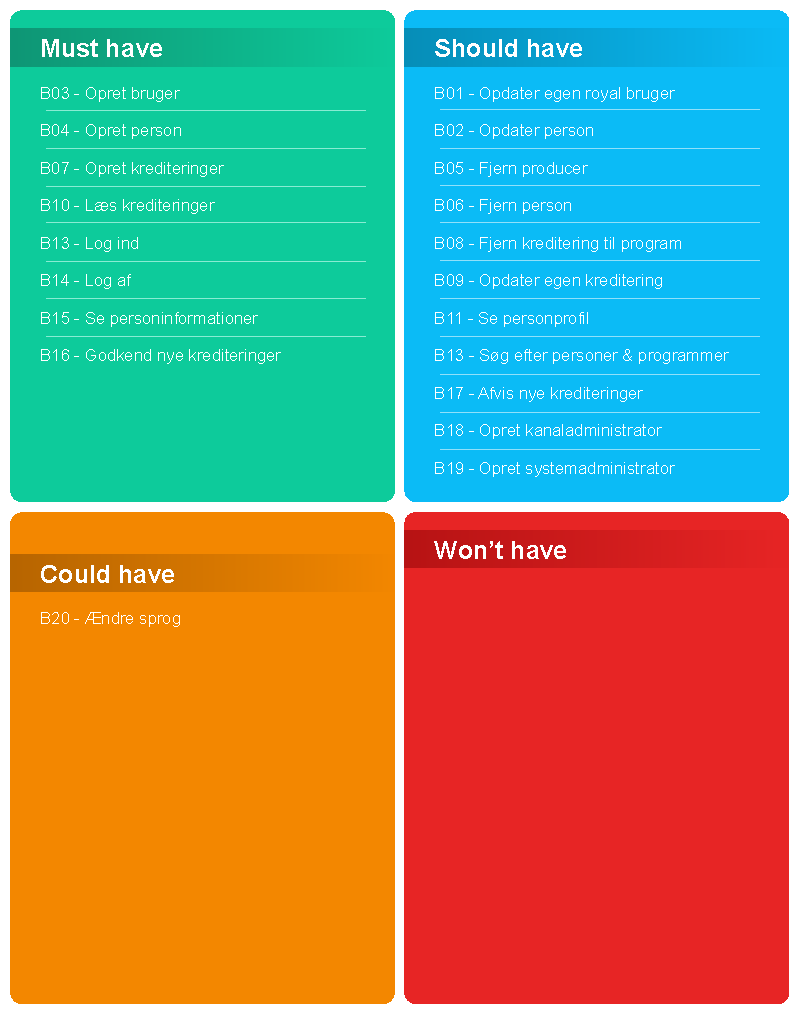
\includegraphics[scale=1]{figures/MoSCoW.pdf}
    \newpage
    
    % Metode i elaborationsfasen
    \section{Metode i elaborationsfasen}


\subsection{UP \& Scrum}

Scrum vil blive brugt i elaborationsfasen, til at nedbryde de krav vi har defineret i inceptionsfasen (se krav). Der vil blive benyttet en sprint periode på 1 uge, da det liner op med det ugentlige vejledermøde. Da sprint perioden er kort (normalt bruges 1-4 uger) er det vigtigt at vi får brudt vores Epics ned til User Stories der kan nåes indenfor 1 sprint.
Vi vil i projektet bruge værktøjet ZenHub til GitHub for at integrere Scrum ind i projektet.
Dette giver os mulighed for at samle vores projekt management og kode inde på vores GitHub side (\url{https://github.com/creditoro}).

\noindent
Vi har til projektet et Kanban board med følgende kolonner:
\begin{itemize}
    \item New Issues
    \item Icebox
    \begin{itemize}
        \item Her er de issues som ikke er prioriteret eller er af lav prioritet (på nuværende tidspunkt).
    \end{itemize}
    \item Backlog
    \begin{itemize}
        \item Kommende issues der er prioriteret højt (sorteret fra top til bund på prioritet).
    \end{itemize}
    \item In Progress
    \begin{itemize}
        \item Hvad der bliver arbejdet på lige nu (sorteret fra top til bund på prioritet).
    \end{itemize}
    \item Done
    \begin{itemize}
        \item Issues der er færdige, disse vil blive lukket til næste sprint møde.
    \end{itemize}
    \item Closed
\end{itemize}

    \newpage
    
    % Ressourcer
    \section{Ressourcer}
I tabel \ref{table:ressourcer} ses det antal timer projektgruppen har samarbejdet om projektet (angivet pr. person). De enkelte medlemmers indsat (læs soloarbejde) er ikke opgjort.\\

\begin{table}[h]
    \centering
    \begin{tabular}{|p{3cm}|p{1cm}|p{1cm}|p{1cm}|p{1cm}|p{1cm}|} 
        \hline
        \textbf{Uge}         & \textbf{7} & \textbf{8} & \textbf{9} & \textbf{10} & \textbf{11}  \\ 
        \hline
        \textbf{Antal timer} & 6          & 11         & 8,5        & 6           & 8            \\ 
        \hline
        \textbf{Timer i alt} & 6          & 17         & 25,5       & 31,5        & 39,9         \\
        \hline
    \end{tabular}
    \caption{Ressourcer brugt på projektet}
    \label{table:ressourcer}
\end{table}

    \newpage
    
    % Konklusion
    \section{Konklusion}
\textit{Opsummering af resultaterne og diskussionen af dem. Svar på om formålet og målene med inceptionsfasen er opnået.}
    \newpage
    
    % Bilag
    \appendix % Bruges til billag, så den laver billag indholdfortegnelse og overskrifter
    \section{Bilag}

\subsection{Logbog}
\href{https://github.com/creditoro/logbook}{\textbf{Logbog} Github.com/creditoro/logbook}

\newpage
\section{Systemsekvensdiagrammer}

% ---------------------------- Opret kreditering ---------------------------------
\begin{figure}[H]
\centering
\includegraphics[scale=0.43]{figures/systemsekvensdiagrammer/opretKreditering.PNG}
\caption{Systemsekvensdiagram for "Opret kreditering"}
\label{fig:create_credit}
\end{figure}

% ---------------------------- Godkend kreditering -------------------------------
\begin{figure}[H]
\centering
\includegraphics[scale=0.43]{figures/systemsekvensdiagrammer/godkendKreditering.PNG}
\caption{Systemsekvensdiagram for "Godkend kreditering"}
\label{fig:approve_credit}
\end{figure}

% ---------------------------- Opret producer ------------------------------------
\begin{figure}[H]
\centering
\includegraphics[scale=0.43]{figures/systemsekvensdiagrammer/opretProducer.PNG}
\caption{Systemsekvensdiagram for "Opret producer"}
\label{fig:create_producer}
\end{figure}

% ---------------------------- Se personinformation ------------------------------
\begin{figure}[H]
\centering
\includegraphics[scale=0.43]{figures/systemsekvensdiagrammer/sePersonInfo.PNG}
\caption{Systemsekvensdiagram for "Se personinformation"}
\label{fig:read_person_info}
\end{figure}

\newpage
\input{appendices/operationssekvensdiagrammer}
\newpage

    \printbibliography
    
\end{document}
